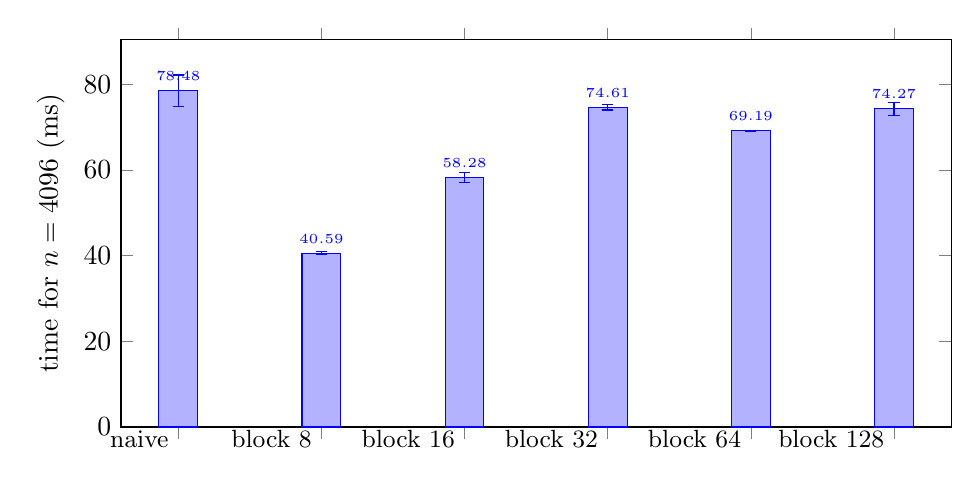
\begin{tikzpicture}
\begin{axis}[ybar, width=\textwidth, height=6.5cm, bar width=14pt, ymin=0, symbolic x coords={naive,block 8,block 16,block 32,block 64,block 128}, xtick=data, x tick label style={rotate=0, anchor=east, font=\small}, ylabel={time for $n = 4096$ (ms)}, enlarge x limits=0.08, legend style={font=\small, at={(0.98,0.98)}, anchor=north east}, nodes near coords, nodes near coords style={font=\tiny}, every node near coord/.append style={/pgf/number format/.cd, fixed, precision=2}]
\addplot+[error bars/.cd, y dir=both, y explicit] coordinates {(naive,78.4800) +- (0,3.6700) (block 8,40.5900) +- (0,0.3700) (block 16,58.2800) +- (0,1.1200) (block 32,74.6100) +- (0,0.6250) (block 64,69.1900) +- (0,0.1050) (block 128,74.2700) +- (0,1.4800)};
\end{axis}
\end{tikzpicture}